\documentclass[11pt,a4paper]{article}
\newcommand{\intestazione}{Trimero ad anello --- 9. Lo scan sui parametri di rumore}
% =====================================================================
%  Preambolo comune ai documenti sul dimero (serie "che cosa abbiamo fatto")
%  Incluso con % =====================================================================
%  Preambolo comune ai documenti sul dimero (serie "che cosa abbiamo fatto")
%  Incluso con % =====================================================================
%  Preambolo comune ai documenti sul dimero (serie "che cosa abbiamo fatto")
%  Incluso con \input{preambolo_dimero} subito dopo \documentclass.
% =====================================================================
\usepackage[T1]{fontenc}
\usepackage[utf8]{inputenc}
\usepackage[main=italian,provide=*]{babel}
\usepackage{amsmath,amssymb,mathtools}
\usepackage{graphicx}
\usepackage{booktabs}
\usepackage{colortbl}
\usepackage{xcolor}
\usepackage{geometry}
\usepackage{placeins}
\usepackage{caption}
\usepackage{enumitem}
\usepackage{fancyhdr}
\usepackage{needspace}
\usepackage{tikz}
\usetikzlibrary{arrows.meta,positioning,shapes.geometric,calc,fit,backgrounds}
\usepackage{hyperref}
\hypersetup{colorlinks=true,linkcolor=blu,citecolor=blu,urlcolor=blu}

\geometry{margin=2.5cm}

% --- colori coerenti con quelli delle figure (palette Okabe-Ito)
\definecolor{blu}{HTML}{0072B2}
\definecolor{arancio}{HTML}{E69F00}
\definecolor{verdes}{HTML}{009E73}
\definecolor{rossos}{HTML}{D55E00}
\definecolor{violas}{HTML}{CC79A7}
\definecolor{grigetto}{HTML}{E8E8E8}

\captionsetup{font=small,labelfont=bf,width=0.92\textwidth}

\pagestyle{fancy}
\fancyhf{}
\fancyhead[L]{\small\itshape\intestazione}
\fancyhead[R]{\small\thepage}
\renewcommand{\headrulewidth}{0.3pt}

% --- notazione
\newcommand{\ket}[1]{\lvert #1\rangle}
\newcommand{\bra}[1]{\langle #1 \rvert}
\newcommand{\media}[1]{\langle #1 \rangle}
\newcommand{\vs}[1]{\mathbf{s}_{#1}}

% --- riquadro "in una riga": il messaggio da portare a casa
\newcommand{\messaggio}[1]{%
  \begin{center}
  \begin{minipage}{0.93\textwidth}
  \setlength{\fboxsep}{9pt}%
  \colorbox{grigetto}{\begin{minipage}{\dimexpr\textwidth-2\fboxsep}
  \small\textbf{In una riga.}\enspace #1
  \end{minipage}}
  \end{minipage}
  \end{center}
}

% --- riquadro "come lo sappiamo": la verifica numerica dietro un'affermazione
\newcommand{\verifica}[1]{%
  \begin{center}
  \begin{minipage}{0.93\textwidth}
  \small\textcolor{verdes}{\rule{2.2em}{1.1pt}}\enspace
  \textcolor{verdes}{\textbf{Come lo sappiamo.}}\enspace #1
  \end{minipage}
  \end{center}
  \medskip
}
 subito dopo \documentclass.
% =====================================================================
\usepackage[T1]{fontenc}
\usepackage[utf8]{inputenc}
\usepackage[main=italian,provide=*]{babel}
\usepackage{amsmath,amssymb,mathtools}
\usepackage{graphicx}
\usepackage{booktabs}
\usepackage{colortbl}
\usepackage{xcolor}
\usepackage{geometry}
\usepackage{placeins}
\usepackage{caption}
\usepackage{enumitem}
\usepackage{fancyhdr}
\usepackage{needspace}
\usepackage{tikz}
\usetikzlibrary{arrows.meta,positioning,shapes.geometric,calc,fit,backgrounds}
\usepackage{hyperref}
\hypersetup{colorlinks=true,linkcolor=blu,citecolor=blu,urlcolor=blu}

\geometry{margin=2.5cm}

% --- colori coerenti con quelli delle figure (palette Okabe-Ito)
\definecolor{blu}{HTML}{0072B2}
\definecolor{arancio}{HTML}{E69F00}
\definecolor{verdes}{HTML}{009E73}
\definecolor{rossos}{HTML}{D55E00}
\definecolor{violas}{HTML}{CC79A7}
\definecolor{grigetto}{HTML}{E8E8E8}

\captionsetup{font=small,labelfont=bf,width=0.92\textwidth}

\pagestyle{fancy}
\fancyhf{}
\fancyhead[L]{\small\itshape\intestazione}
\fancyhead[R]{\small\thepage}
\renewcommand{\headrulewidth}{0.3pt}

% --- notazione
\newcommand{\ket}[1]{\lvert #1\rangle}
\newcommand{\bra}[1]{\langle #1 \rvert}
\newcommand{\media}[1]{\langle #1 \rangle}
\newcommand{\vs}[1]{\mathbf{s}_{#1}}

% --- riquadro "in una riga": il messaggio da portare a casa
\newcommand{\messaggio}[1]{%
  \begin{center}
  \begin{minipage}{0.93\textwidth}
  \setlength{\fboxsep}{9pt}%
  \colorbox{grigetto}{\begin{minipage}{\dimexpr\textwidth-2\fboxsep}
  \small\textbf{In una riga.}\enspace #1
  \end{minipage}}
  \end{minipage}
  \end{center}
}

% --- riquadro "come lo sappiamo": la verifica numerica dietro un'affermazione
\newcommand{\verifica}[1]{%
  \begin{center}
  \begin{minipage}{0.93\textwidth}
  \small\textcolor{verdes}{\rule{2.2em}{1.1pt}}\enspace
  \textcolor{verdes}{\textbf{Come lo sappiamo.}}\enspace #1
  \end{minipage}
  \end{center}
  \medskip
}
 subito dopo \documentclass.
% =====================================================================
\usepackage[T1]{fontenc}
\usepackage[utf8]{inputenc}
\usepackage[main=italian,provide=*]{babel}
\usepackage{amsmath,amssymb,mathtools}
\usepackage{graphicx}
\usepackage{booktabs}
\usepackage{colortbl}
\usepackage{xcolor}
\usepackage{geometry}
\usepackage{placeins}
\usepackage{caption}
\usepackage{enumitem}
\usepackage{fancyhdr}
\usepackage{needspace}
\usepackage{tikz}
\usetikzlibrary{arrows.meta,positioning,shapes.geometric,calc,fit,backgrounds}
\usepackage{hyperref}
\hypersetup{colorlinks=true,linkcolor=blu,citecolor=blu,urlcolor=blu}

\geometry{margin=2.5cm}

% --- colori coerenti con quelli delle figure (palette Okabe-Ito)
\definecolor{blu}{HTML}{0072B2}
\definecolor{arancio}{HTML}{E69F00}
\definecolor{verdes}{HTML}{009E73}
\definecolor{rossos}{HTML}{D55E00}
\definecolor{violas}{HTML}{CC79A7}
\definecolor{grigetto}{HTML}{E8E8E8}

\captionsetup{font=small,labelfont=bf,width=0.92\textwidth}

\pagestyle{fancy}
\fancyhf{}
\fancyhead[L]{\small\itshape\intestazione}
\fancyhead[R]{\small\thepage}
\renewcommand{\headrulewidth}{0.3pt}

% --- notazione
\newcommand{\ket}[1]{\lvert #1\rangle}
\newcommand{\bra}[1]{\langle #1 \rvert}
\newcommand{\media}[1]{\langle #1 \rangle}
\newcommand{\vs}[1]{\mathbf{s}_{#1}}

% --- riquadro "in una riga": il messaggio da portare a casa
\newcommand{\messaggio}[1]{%
  \begin{center}
  \begin{minipage}{0.93\textwidth}
  \setlength{\fboxsep}{9pt}%
  \colorbox{grigetto}{\begin{minipage}{\dimexpr\textwidth-2\fboxsep}
  \small\textbf{In una riga.}\enspace #1
  \end{minipage}}
  \end{minipage}
  \end{center}
}

% --- riquadro "come lo sappiamo": la verifica numerica dietro un'affermazione
\newcommand{\verifica}[1]{%
  \begin{center}
  \begin{minipage}{0.93\textwidth}
  \small\textcolor{verdes}{\rule{2.2em}{1.1pt}}\enspace
  \textcolor{verdes}{\textbf{Come lo sappiamo.}}\enspace #1
  \end{minipage}
  \end{center}
  \medskip
}


\title{\bfseries Un solo chip non basta a dire qualcosa di generale\\[2pt]
\large Documento 9 --- come si sposta $N^*$ al variare del rumore}
\author{Samuele Schiavi \\ \small Tesi triennale in Fisica, Università di Parma
--- Relatore: Prof.\ Alessandro Chiesa}
\date{}

\begin{document}
\maketitle
\thispagestyle{fancy}

\section{Perché non fermarsi al punto di calibrazione}

I Documenti 7 e 8 danno $N^*$ a un solo punto (\texttt{ibm\_torino}). Un
chip diverso, o lo stesso chip fra qualche mese, avrebbe parametri diversi
--- serve sapere come $N^*$ si sposta, non solo il suo valore in un punto.

\section{Monotonia rispetto al rumore di gate}

\begin{figure}[htbp]
\centering
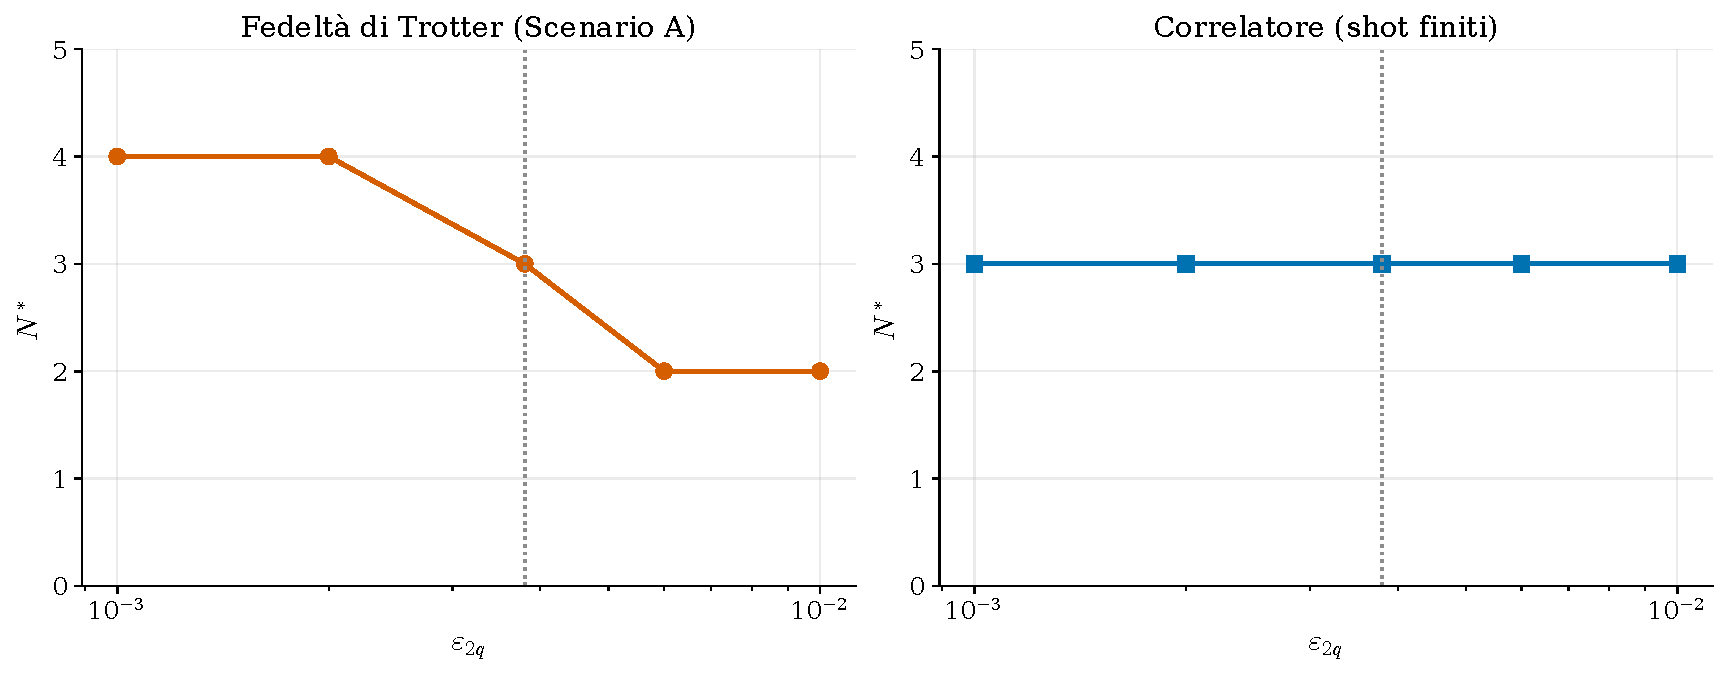
\includegraphics[width=\textwidth]{figure/fig_passo5_Nstar_vs_eps_anello}
\caption{$N^*$ in funzione di $\varepsilon_{2q}$ (scala logaritmica),
$\varepsilon_{1q}$ e $p_\text{readout}$ fissati al riferimento.
\textbf{Sinistra}: fedeltà di Trotter (Scenario A, $b/J=2.4$,
$D/J=0.15$). \textbf{Destra}:
correlatore, readout a shot finiti. Entrambe monotone non-crescenti, come
atteso: più rumore, meno conviene allungare il circuito.}
\end{figure}
\FloatBarrier

\begin{table}[htbp]
\centering
\small
\renewcommand{\arraystretch}{1.3}
\begin{tabular}{@{}lccc@{}}
\toprule
\rowcolor{grigetto}
$\varepsilon_{2q}$ & $N^*$ Trotter & $N^*$ correlatore \\
\midrule
$1\times10^{-3}$ & 4 & 3 \\
$2\times10^{-3}$ & 4 & 3 \\
$3.8\times10^{-3}$ (riferimento) & 3 & 3 \\
$6\times10^{-3}$ & 2 & 3 \\
$1\times10^{-2}$ & 2 & 3 \\
\bottomrule
\end{tabular}
\caption{$N^*$ Trotter scende con $\varepsilon_{2q}$; $N^*$ correlatore
resta fermo a $3$ su tutto il range esplorato --- una differenza fra le due
metriche non vista in questa forma sul dimero, dove entrambe scendevano
in modo comparabile. Non ancora indagata la ragione: dichiarata come
osservazione aperta, non forzata in una spiegazione.}
\end{table}
\FloatBarrier

\section{Invarianza rispetto al readout}

\verifica{$N^*$ del correlatore, a shot finiti, su tre valori di
$p_\text{readout}$: $0.00\to N^*=3$; $0.05\to N^*=3$; $0.20\to N^*=3$ ---
invariato, verificato numericamente con una misura vera, non solo assunto
dall'argomento analitico (che pure vale: la correzione di readout
simmetrico è un fattore moltiplicativo costante in $N$, non può spostare
un massimo).}

\messaggio{L'invarianza da $p_\text{readout}$ non è una sorpresa --- è
dimostrata in generale per il caso simmetrico, sul dimero come qui. La
parte verificata qui, non garantita a priori, è che la dimostrazione regga
anche quando il readout è implementato come misura vera a shot finiti, non
come formula.}

\section{Cosa non copre questo scan}

\begin{itemize}[leftmargin=1.5em,itemsep=2pt]
\item Nessuna combinazione congiunta $(\varepsilon_{1q},\varepsilon_{2q})$
esplorata simultaneamente --- un parametro alla volta, l'altro fissato al
riferimento.
\item Il punto $R_0$ (Scenario B) non è ripreso in questo scan: solo lo
Scenario A.
\end{itemize}

\section{Dove chiude questa parte della pipeline}

I cinque stadi (Documenti 5--9) sono ora chiusi. Le due estensioni che
seguono (Documenti 10, 11) non sono richieste, ma rispondono a due domande
lasciate aperte: vale la pena riottimizzare vedendo il rumore? E cosa
succede quando il readout smette di essere simmetrico?

\end{document}
